\documentclass[twoside]{book}

% Packages required by doxygen
\usepackage{fixltx2e}
\usepackage{calc}
\usepackage{doxygen}
\usepackage[export]{adjustbox} % also loads graphicx
\usepackage{graphicx}
\usepackage[utf8]{inputenc}
\usepackage{makeidx}
\usepackage{multicol}
\usepackage{multirow}
\PassOptionsToPackage{warn}{textcomp}
\usepackage{textcomp}
\usepackage[nointegrals]{wasysym}
\usepackage[table]{xcolor}

% Font selection
\usepackage[T1]{fontenc}
\usepackage[scaled=.90]{helvet}
\usepackage{courier}
\usepackage{amssymb}
\usepackage{sectsty}
\renewcommand{\familydefault}{\sfdefault}
\allsectionsfont{%
  \fontseries{bc}\selectfont%
  \color{darkgray}%
}
\renewcommand{\DoxyLabelFont}{%
  \fontseries{bc}\selectfont%
  \color{darkgray}%
}
\newcommand{\+}{\discretionary{\mbox{\scriptsize$\hookleftarrow$}}{}{}}

% Page & text layout
\usepackage{geometry}
\geometry{%
  a4paper,%
  top=2.5cm,%
  bottom=2.5cm,%
  left=2.5cm,%
  right=2.5cm%
}
\tolerance=750
\hfuzz=15pt
\hbadness=750
\setlength{\emergencystretch}{15pt}
\setlength{\parindent}{0cm}
\setlength{\parskip}{3ex plus 2ex minus 2ex}
\makeatletter
\renewcommand{\paragraph}{%
  \@startsection{paragraph}{4}{0ex}{-1.0ex}{1.0ex}{%
    \normalfont\normalsize\bfseries\SS@parafont%
  }%
}
\renewcommand{\subparagraph}{%
  \@startsection{subparagraph}{5}{0ex}{-1.0ex}{1.0ex}{%
    \normalfont\normalsize\bfseries\SS@subparafont%
  }%
}
\makeatother

% Headers & footers
\usepackage{fancyhdr}
\pagestyle{fancyplain}
\fancyhead[LE]{\fancyplain{}{\bfseries\thepage}}
\fancyhead[CE]{\fancyplain{}{}}
\fancyhead[RE]{\fancyplain{}{\bfseries\leftmark}}
\fancyhead[LO]{\fancyplain{}{\bfseries\rightmark}}
\fancyhead[CO]{\fancyplain{}{}}
\fancyhead[RO]{\fancyplain{}{\bfseries\thepage}}
\fancyfoot[LE]{\fancyplain{}{}}
\fancyfoot[CE]{\fancyplain{}{}}
\fancyfoot[RE]{\fancyplain{}{\bfseries\scriptsize Generated by Doxygen }}
\fancyfoot[LO]{\fancyplain{}{\bfseries\scriptsize Generated by Doxygen }}
\fancyfoot[CO]{\fancyplain{}{}}
\fancyfoot[RO]{\fancyplain{}{}}
\renewcommand{\footrulewidth}{0.4pt}
\renewcommand{\chaptermark}[1]{%
  \markboth{#1}{}%
}
\renewcommand{\sectionmark}[1]{%
  \markright{\thesection\ #1}%
}

% Indices & bibliography
\usepackage{natbib}
\usepackage[titles]{tocloft}
\setcounter{tocdepth}{3}
\setcounter{secnumdepth}{5}
\makeindex

% Hyperlinks (required, but should be loaded last)
\usepackage{ifpdf}
\ifpdf
  \usepackage[pdftex,pagebackref=true]{hyperref}
\else
  \usepackage[ps2pdf,pagebackref=true]{hyperref}
\fi
\hypersetup{%
  colorlinks=true,%
  linkcolor=blue,%
  citecolor=blue,%
  unicode%
}

% Custom commands
\newcommand{\clearemptydoublepage}{%
  \newpage{\pagestyle{empty}\cleardoublepage}%
}

\usepackage{caption}
\captionsetup{labelsep=space,justification=centering,font={bf},singlelinecheck=off,skip=4pt,position=top}

%===== C O N T E N T S =====

\begin{document}

% Titlepage & ToC
\hypersetup{pageanchor=false,
             bookmarksnumbered=true,
             pdfencoding=unicode
            }
\pagenumbering{alph}
\begin{titlepage}
\vspace*{7cm}
\begin{center}%
{\Large My Project }\\
\vspace*{1cm}
{\large Generated by Doxygen 1.8.14}\\
\end{center}
\end{titlepage}
\clearemptydoublepage
\pagenumbering{roman}
\tableofcontents
\clearemptydoublepage
\pagenumbering{arabic}
\hypersetup{pageanchor=true}

%--- Begin generated contents ---
\chapter{Namespace Index}
\section{Namespace List}
Here is a list of all documented namespaces with brief descriptions\+:\begin{DoxyCompactList}
\item\contentsline{section}{\mbox{\hyperlink{namespace_completed}{Completed}} }{\pageref{namespace_completed}}{}
\end{DoxyCompactList}

\chapter{Hierarchical Index}
\section{Class Hierarchy}
This inheritance list is sorted roughly, but not completely, alphabetically\+:\begin{DoxyCompactList}
\item I\+Player\begin{DoxyCompactList}
\item \contentsline{section}{Gingy}{\pageref{class_gingy}}{}
\end{DoxyCompactList}
\item Mono\+Behaviour\begin{DoxyCompactList}
\item \contentsline{section}{Camera\+Follow}{\pageref{class_camera_follow}}{}
\item \contentsline{section}{Completed.\+Level\+Generator}{\pageref{class_completed_1_1_level_generator}}{}
\item \contentsline{section}{Enemy\+AI}{\pageref{class_enemy_a_i}}{}
\item \contentsline{section}{Game\+Manager}{\pageref{class_game_manager}}{}
\item \contentsline{section}{Game\+Over}{\pageref{class_game_over}}{}
\item \contentsline{section}{Loader}{\pageref{class_loader}}{}
\item \contentsline{section}{Main\+Menu}{\pageref{class_main_menu}}{}
\item \contentsline{section}{Map}{\pageref{class_map}}{}
\end{DoxyCompactList}
\end{DoxyCompactList}

\chapter{Class Index}
\section{Class List}
Here are the classes, structs, unions and interfaces with brief descriptions\+:\begin{DoxyCompactList}
\item\contentsline{section}{\mbox{\hyperlink{class_camera_follow}{Camera\+Follow}} }{\pageref{class_camera_follow}}{}
\item\contentsline{section}{\mbox{\hyperlink{class_enemy_a_i}{Enemy\+AI}} }{\pageref{class_enemy_a_i}}{}
\item\contentsline{section}{\mbox{\hyperlink{class_game_manager}{Game\+Manager}} }{\pageref{class_game_manager}}{}
\item\contentsline{section}{\mbox{\hyperlink{class_game_over}{Game\+Over}} }{\pageref{class_game_over}}{}
\item\contentsline{section}{\mbox{\hyperlink{class_gingy}{Gingy}} }{\pageref{class_gingy}}{}
\item\contentsline{section}{\mbox{\hyperlink{class_completed_1_1_level_generator}{Completed.\+Level\+Generator}} }{\pageref{class_completed_1_1_level_generator}}{}
\item\contentsline{section}{\mbox{\hyperlink{class_loader}{Loader}} }{\pageref{class_loader}}{}
\item\contentsline{section}{\mbox{\hyperlink{class_main_menu}{Main\+Menu}} }{\pageref{class_main_menu}}{}
\item\contentsline{section}{\mbox{\hyperlink{class_map}{Map}} }{\pageref{class_map}}{}
\end{DoxyCompactList}

\chapter{Namespace Documentation}
\hypertarget{namespace_completed}{}\section{Completed Namespace Reference}
\label{namespace_completed}\index{Completed@{Completed}}
\subsection*{Classes}
\begin{DoxyCompactItemize}
\item 
class \mbox{\hyperlink{class_completed_1_1_level_generator}{Level\+Generator}}
\end{DoxyCompactItemize}

\chapter{Class Documentation}
\hypertarget{class_camera_follow}{}\section{Camera\+Follow Class Reference}
\label{class_camera_follow}\index{Camera\+Follow@{Camera\+Follow}}
Inheritance diagram for Camera\+Follow\+:\begin{figure}[H]
\begin{center}
\leavevmode
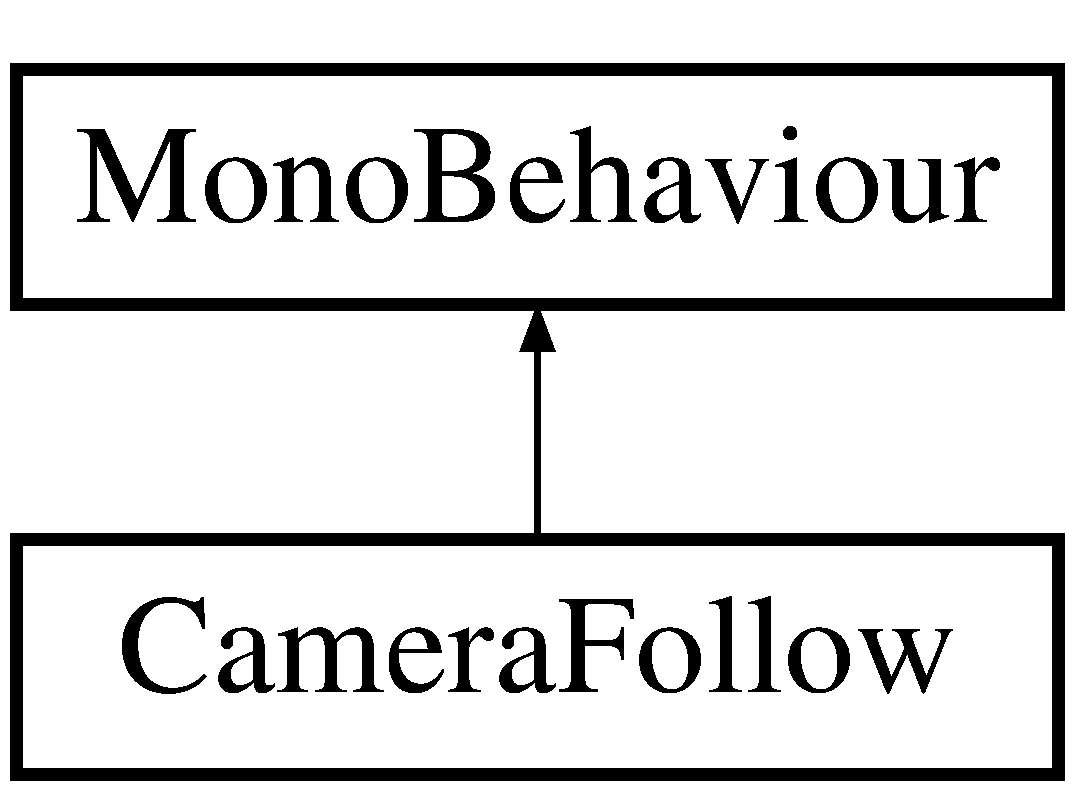
\includegraphics[height=2.000000cm]{class_camera_follow}
\end{center}
\end{figure}
\subsection*{Public Attributes}
\begin{DoxyCompactItemize}
\item 
\mbox{\Hypertarget{class_camera_follow_a2ef2d3655fd0cb86d18e6324b75c0a59}\label{class_camera_follow_a2ef2d3655fd0cb86d18e6324b75c0a59}} 
Transform {\bfseries target}
\item 
\mbox{\Hypertarget{class_camera_follow_a924c2f26a261004c89aa63ca0c89d454}\label{class_camera_follow_a924c2f26a261004c89aa63ca0c89d454}} 
float {\bfseries smooth\+Speed} = 0.\+125f
\end{DoxyCompactItemize}


The documentation for this class was generated from the following file\+:\begin{DoxyCompactItemize}
\item 
Camera\+Follow.\+cs\end{DoxyCompactItemize}

\hypertarget{class_enemy_a_i}{}\section{Enemy\+AI Class Reference}
\label{class_enemy_a_i}\index{Enemy\+AI@{Enemy\+AI}}
Inheritance diagram for Enemy\+AI\+:\begin{figure}[H]
\begin{center}
\leavevmode
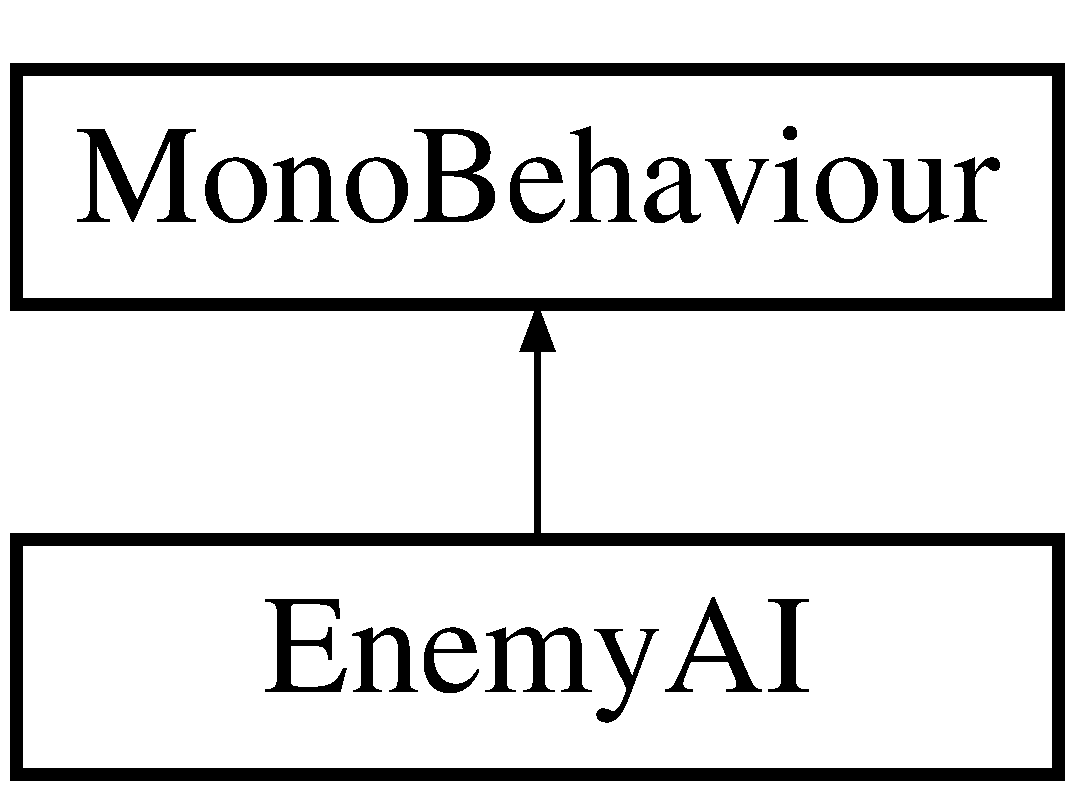
\includegraphics[height=2.000000cm]{class_enemy_a_i}
\end{center}
\end{figure}
\subsection*{Public Member Functions}
\begin{DoxyCompactItemize}
\item 
void \mbox{\hyperlink{class_enemy_a_i_aa199fde66aef59a3ca5898fefa699ca8}{try\+Attack}} ()
\item 
\mbox{\Hypertarget{class_enemy_a_i_a6043590f1a68dee54de9e8f599cad88d}\label{class_enemy_a_i_a6043590f1a68dee54de9e8f599cad88d}} 
void {\bfseries toggle\+Move} ()
\end{DoxyCompactItemize}
\subsection*{Public Attributes}
\begin{DoxyCompactItemize}
\item 
\mbox{\Hypertarget{class_enemy_a_i_a415f57823bb4f2490f98bedb56ae6b49}\label{class_enemy_a_i_a415f57823bb4f2490f98bedb56ae6b49}} 
Game\+Object {\bfseries Player}
\end{DoxyCompactItemize}


\subsection{Member Function Documentation}
\mbox{\Hypertarget{class_enemy_a_i_aa199fde66aef59a3ca5898fefa699ca8}\label{class_enemy_a_i_aa199fde66aef59a3ca5898fefa699ca8}} 
\index{Enemy\+AI@{Enemy\+AI}!try\+Attack@{try\+Attack}}
\index{try\+Attack@{try\+Attack}!Enemy\+AI@{Enemy\+AI}}
\subsubsection{\texorpdfstring{try\+Attack()}{tryAttack()}}
{\footnotesize\ttfamily void Enemy\+A\+I.\+try\+Attack (\begin{DoxyParamCaption}{ }\end{DoxyParamCaption})\hspace{0.3cm}{\ttfamily [inline]}}

Attempts to attack the main player within a certain radius.  None  None 

The documentation for this class was generated from the following file\+:\begin{DoxyCompactItemize}
\item 
Enemy\+A\+I.\+cs\end{DoxyCompactItemize}

\hypertarget{class_game_manager}{}\section{Game\+Manager Class Reference}
\label{class_game_manager}\index{Game\+Manager@{Game\+Manager}}
Inheritance diagram for Game\+Manager\+:\begin{figure}[H]
\begin{center}
\leavevmode
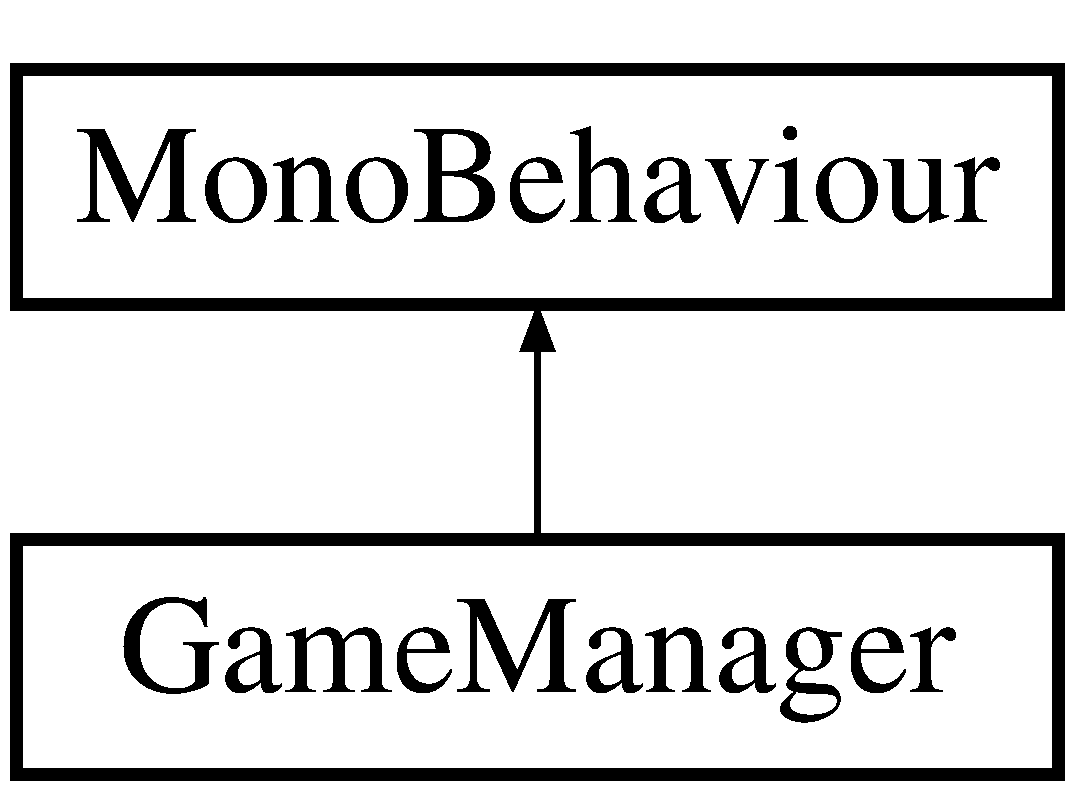
\includegraphics[height=2.000000cm]{class_game_manager}
\end{center}
\end{figure}
\subsection*{Public Attributes}
\begin{DoxyCompactItemize}
\item 
\mbox{\Hypertarget{class_game_manager_a2195c4ae8d753a31d968d7c8347668de}\label{class_game_manager_a2195c4ae8d753a31d968d7c8347668de}} 
float {\bfseries level\+Start\+Delay} = 2f
\item 
\mbox{\Hypertarget{class_game_manager_a80dd88e2622249f02c752fc84cac3f92}\label{class_game_manager_a80dd88e2622249f02c752fc84cac3f92}} 
\mbox{\hyperlink{class_completed_1_1_level_generator}{Level\+Generator}} {\bfseries level\+Generator}
\item 
\mbox{\Hypertarget{class_game_manager_a6b205783f48dd535e8db182d69e55ed7}\label{class_game_manager_a6b205783f48dd535e8db182d69e55ed7}} 
Game\+Object {\bfseries main\+Character}
\end{DoxyCompactItemize}
\subsection*{Static Public Attributes}
\begin{DoxyCompactItemize}
\item 
\mbox{\Hypertarget{class_game_manager_a7666e8468dac197b9eb32dd32128524f}\label{class_game_manager_a7666e8468dac197b9eb32dd32128524f}} 
static \mbox{\hyperlink{class_game_manager}{Game\+Manager}} {\bfseries instance} = null
\end{DoxyCompactItemize}


The documentation for this class was generated from the following file\+:\begin{DoxyCompactItemize}
\item 
Game\+Manager.\+cs\end{DoxyCompactItemize}

\hypertarget{class_game_over}{}\section{Game\+Over Class Reference}
\label{class_game_over}\index{Game\+Over@{Game\+Over}}
Inheritance diagram for Game\+Over\+:\begin{figure}[H]
\begin{center}
\leavevmode
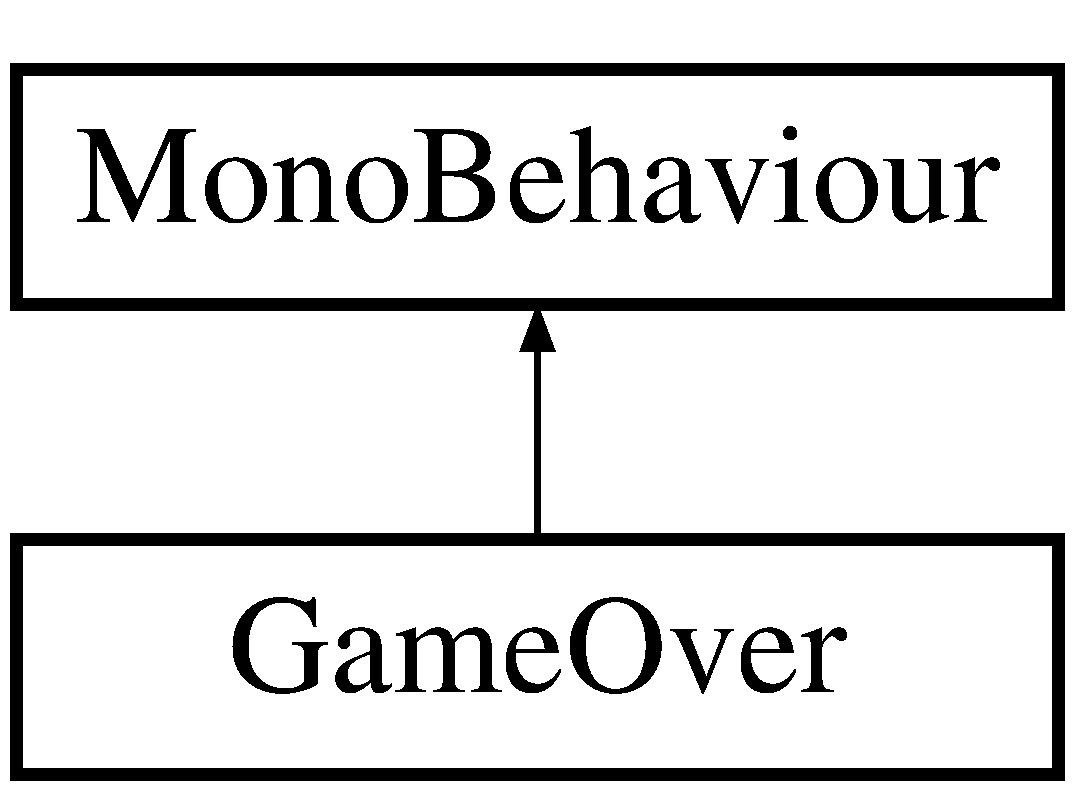
\includegraphics[height=2.000000cm]{class_game_over}
\end{center}
\end{figure}
\subsection*{Public Member Functions}
\begin{DoxyCompactItemize}
\item 
void \mbox{\hyperlink{class_game_over_af7a0b3719580737182a952c8fb487232}{to\+Main\+Menu}} ()
\end{DoxyCompactItemize}


\subsection{Member Function Documentation}
\mbox{\Hypertarget{class_game_over_af7a0b3719580737182a952c8fb487232}\label{class_game_over_af7a0b3719580737182a952c8fb487232}} 
\index{Game\+Over@{Game\+Over}!to\+Main\+Menu@{to\+Main\+Menu}}
\index{to\+Main\+Menu@{to\+Main\+Menu}!Game\+Over@{Game\+Over}}
\subsubsection{\texorpdfstring{to\+Main\+Menu()}{toMainMenu()}}
{\footnotesize\ttfamily void Game\+Over.\+to\+Main\+Menu (\begin{DoxyParamCaption}{ }\end{DoxyParamCaption})\hspace{0.3cm}{\ttfamily [inline]}}

Loads \mbox{\hyperlink{class_main_menu}{Main\+Menu}}  None  None 

The documentation for this class was generated from the following file\+:\begin{DoxyCompactItemize}
\item 
Game\+Over.\+cs\end{DoxyCompactItemize}

\hypertarget{class_gingy}{}\section{Gingy Class Reference}
\label{class_gingy}\index{Gingy@{Gingy}}
Inheritance diagram for Gingy\+:\begin{figure}[H]
\begin{center}
\leavevmode
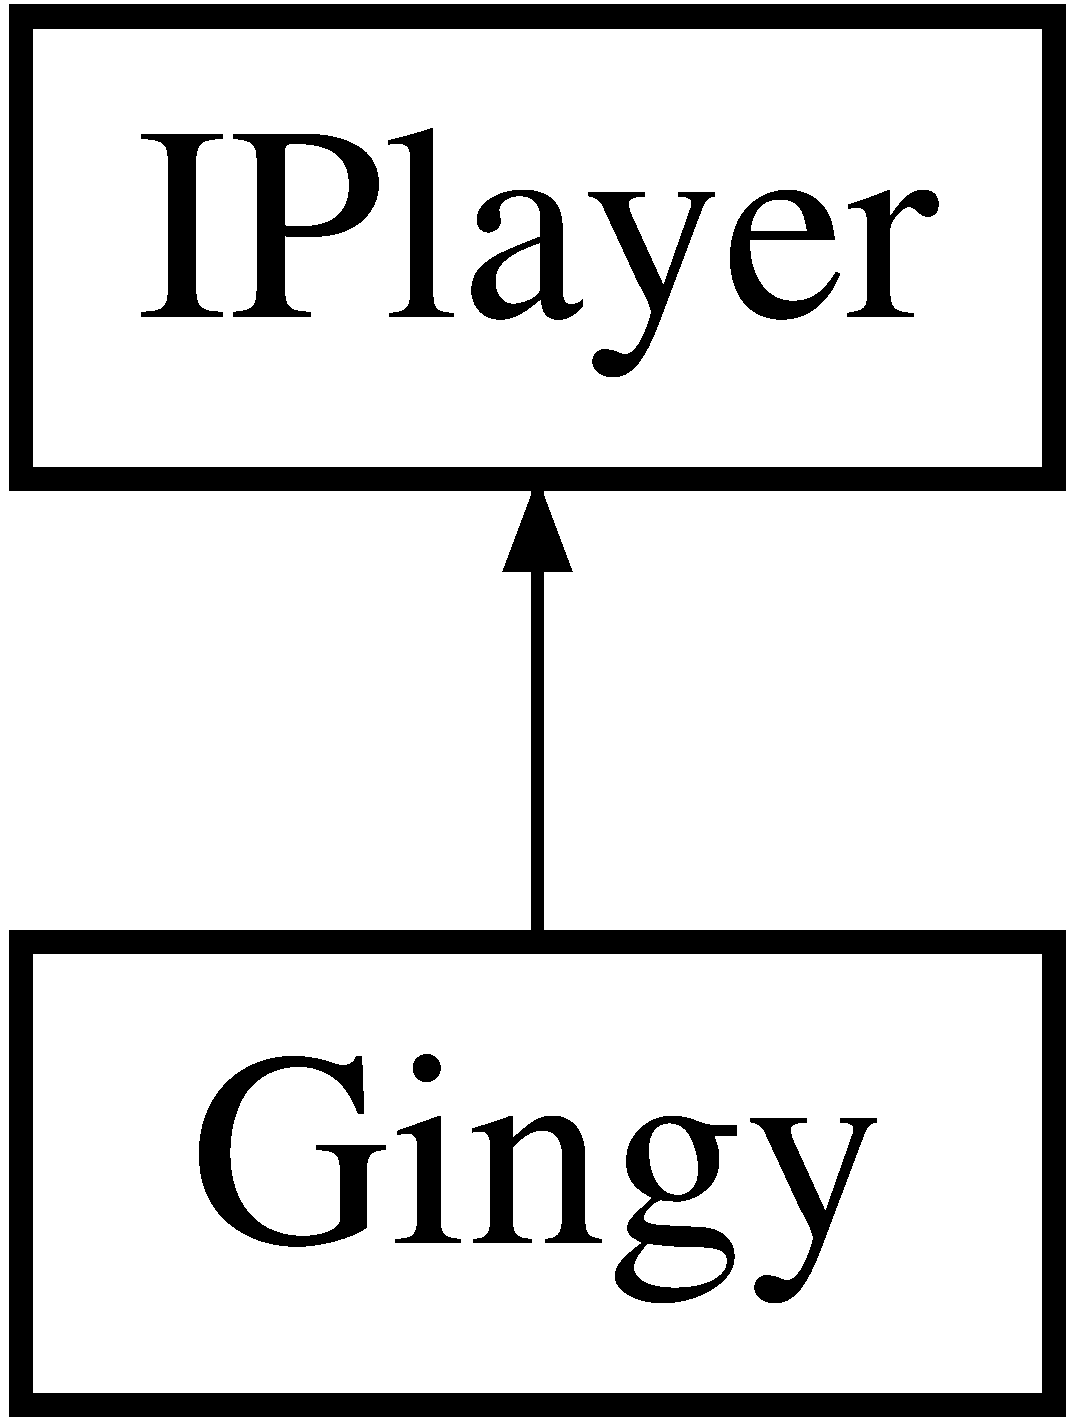
\includegraphics[height=2.000000cm]{class_gingy}
\end{center}
\end{figure}
\subsection*{Public Attributes}
\begin{DoxyCompactItemize}
\item 
\mbox{\Hypertarget{class_gingy_a1f2c2d5434afa46ac7c79e4a6eaa4fd5}\label{class_gingy_a1f2c2d5434afa46ac7c79e4a6eaa4fd5}} 
int {\bfseries Health} = 100
\end{DoxyCompactItemize}


The documentation for this class was generated from the following file\+:\begin{DoxyCompactItemize}
\item 
Gingy.\+cs\end{DoxyCompactItemize}

\hypertarget{class_completed_1_1_level_generator}{}\section{Completed.\+Level\+Generator Class Reference}
\label{class_completed_1_1_level_generator}\index{Completed.\+Level\+Generator@{Completed.\+Level\+Generator}}
Inheritance diagram for Completed.\+Level\+Generator\+:\begin{figure}[H]
\begin{center}
\leavevmode
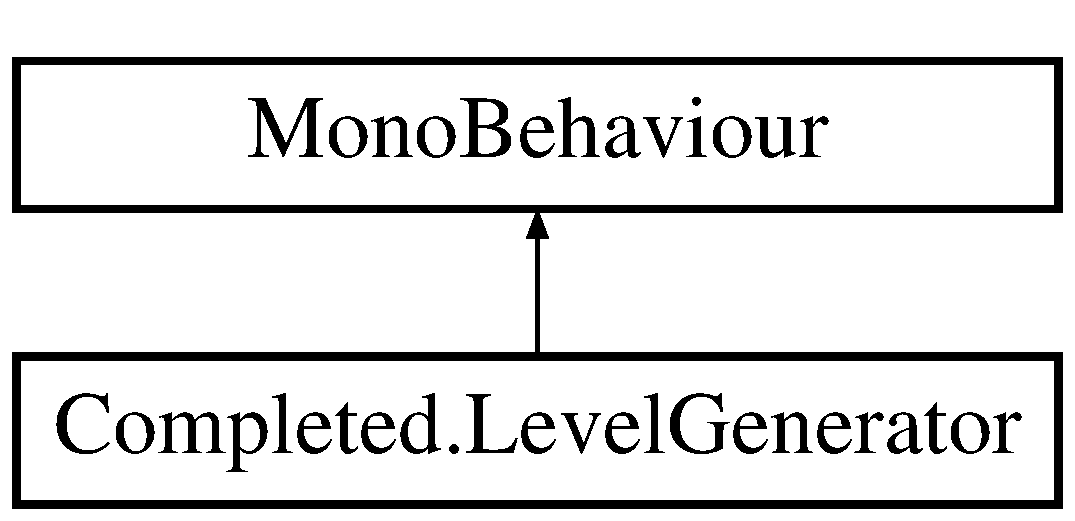
\includegraphics[height=2.000000cm]{class_completed_1_1_level_generator}
\end{center}
\end{figure}
\subsection*{Public Member Functions}
\begin{DoxyCompactItemize}
\item 
\mbox{\Hypertarget{class_completed_1_1_level_generator_aa6cf39de7260a0ac492e31dbc6c8273a}\label{class_completed_1_1_level_generator_aa6cf39de7260a0ac492e31dbc6c8273a}} 
void {\bfseries Setup\+Scene} (int level)
\item 
\mbox{\Hypertarget{class_completed_1_1_level_generator_a1738146aa2a12138c19070b4bdbc2d22}\label{class_completed_1_1_level_generator_a1738146aa2a12138c19070b4bdbc2d22}} 
void {\bfseries Place\+Player} (Game\+Object Player)
\item 
\mbox{\Hypertarget{class_completed_1_1_level_generator_a2ffea5be00328c47fa5460db2386b8e5}\label{class_completed_1_1_level_generator_a2ffea5be00328c47fa5460db2386b8e5}} 
int {\bfseries get\+Num\+Enemies} ()
\end{DoxyCompactItemize}
\subsection*{Public Attributes}
\begin{DoxyCompactItemize}
\item 
\mbox{\Hypertarget{class_completed_1_1_level_generator_a1f495bac99f2520a6cdc7949abd1901a}\label{class_completed_1_1_level_generator_a1f495bac99f2520a6cdc7949abd1901a}} 
int {\bfseries placed\+Floors}
\item 
\mbox{\Hypertarget{class_completed_1_1_level_generator_a4d3a79f611c1f1958372a9fa018fef12}\label{class_completed_1_1_level_generator_a4d3a79f611c1f1958372a9fa018fef12}} 
int {\bfseries num\+Floor\+Tiles}
\item 
\mbox{\Hypertarget{class_completed_1_1_level_generator_a3683acf37342e58917d62bdfb4920605}\label{class_completed_1_1_level_generator_a3683acf37342e58917d62bdfb4920605}} 
\mbox{\hyperlink{class_map}{Map}} {\bfseries map}
\item 
\mbox{\Hypertarget{class_completed_1_1_level_generator_a96a5d7a791a7cace1db5fac4932bd0a3}\label{class_completed_1_1_level_generator_a96a5d7a791a7cace1db5fac4932bd0a3}} 
int {\bfseries num\+Items}
\item 
\mbox{\Hypertarget{class_completed_1_1_level_generator_a285945bcaa4e52d34b86ffc0c5492d60}\label{class_completed_1_1_level_generator_a285945bcaa4e52d34b86ffc0c5492d60}} 
Game\+Object \mbox{[}$\,$\mbox{]} {\bfseries Items}
\item 
\mbox{\Hypertarget{class_completed_1_1_level_generator_ab820dfc29b9b876659a155b7e72dcc15}\label{class_completed_1_1_level_generator_ab820dfc29b9b876659a155b7e72dcc15}} 
Vector3 {\bfseries player\+Pos}
\item 
\mbox{\Hypertarget{class_completed_1_1_level_generator_a45c4fdc5051944c5036fa56e8ad85ae1}\label{class_completed_1_1_level_generator_a45c4fdc5051944c5036fa56e8ad85ae1}} 
Game\+Object {\bfseries Enemy}
\item 
\mbox{\Hypertarget{class_completed_1_1_level_generator_acb8af6a600d1121e4d1e55c8b827d4ff}\label{class_completed_1_1_level_generator_acb8af6a600d1121e4d1e55c8b827d4ff}} 
int {\bfseries num\+Enemies}
\end{DoxyCompactItemize}


The documentation for this class was generated from the following file\+:\begin{DoxyCompactItemize}
\item 
Level\+Generator.\+cs\end{DoxyCompactItemize}

\hypertarget{class_loader}{}\section{Loader Class Reference}
\label{class_loader}\index{Loader@{Loader}}
Inheritance diagram for Loader\+:\begin{figure}[H]
\begin{center}
\leavevmode
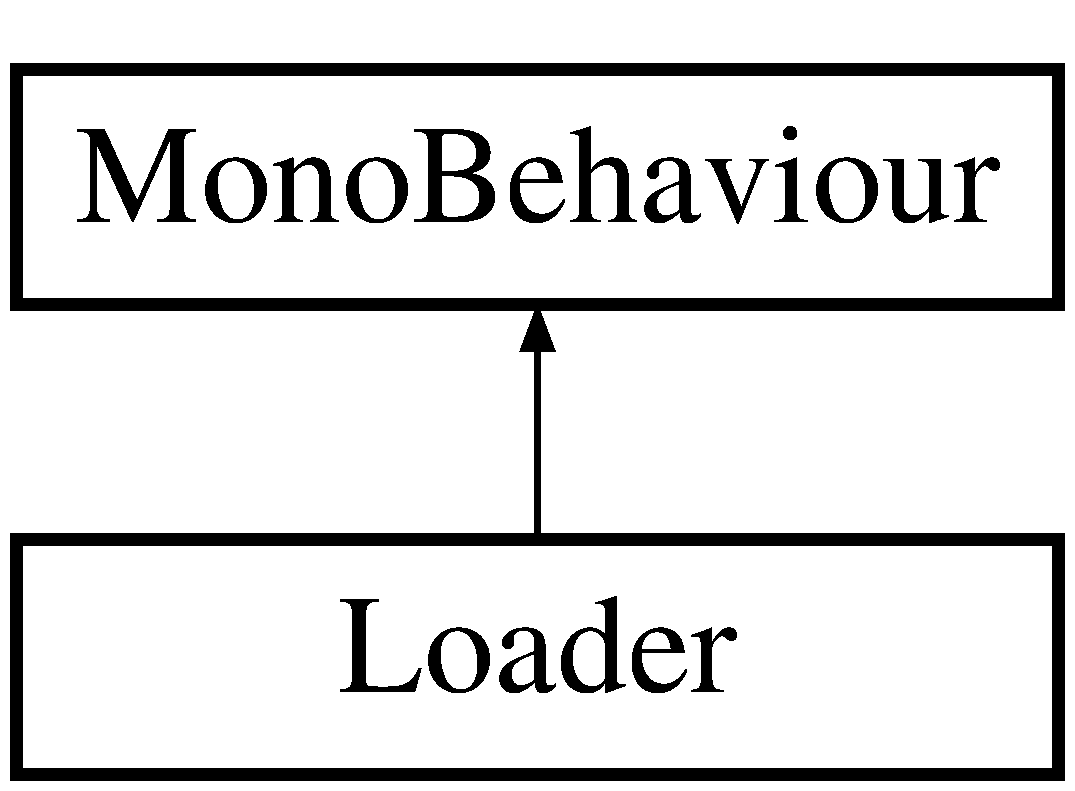
\includegraphics[height=2.000000cm]{class_loader}
\end{center}
\end{figure}
\subsection*{Public Attributes}
\begin{DoxyCompactItemize}
\item 
\mbox{\Hypertarget{class_loader_a4eee44244b0fa6a5708e2ffbee772403}\label{class_loader_a4eee44244b0fa6a5708e2ffbee772403}} 
\mbox{\hyperlink{class_game_manager}{Game\+Manager}} {\bfseries game\+Manager}
\end{DoxyCompactItemize}


The documentation for this class was generated from the following file\+:\begin{DoxyCompactItemize}
\item 
Loader.\+cs\end{DoxyCompactItemize}

\hypertarget{class_main_menu}{}\section{Main\+Menu Class Reference}
\label{class_main_menu}\index{Main\+Menu@{Main\+Menu}}
Inheritance diagram for Main\+Menu\+:\begin{figure}[H]
\begin{center}
\leavevmode
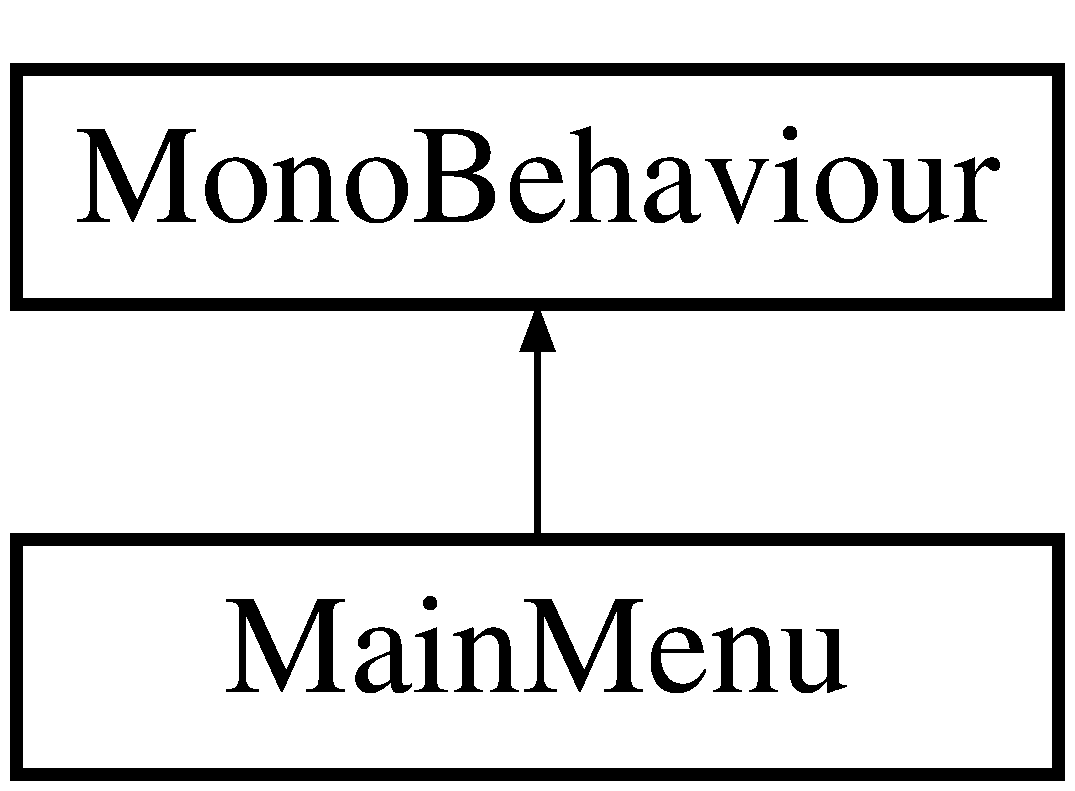
\includegraphics[height=2.000000cm]{class_main_menu}
\end{center}
\end{figure}
\subsection*{Public Member Functions}
\begin{DoxyCompactItemize}
\item 
void \mbox{\hyperlink{class_main_menu_a11d7e3cd6b90cf59659e03e830e02db5}{Play\+Game}} ()
\item 
void \mbox{\hyperlink{class_main_menu_a485db7cf60c0b93ecc87b9273bcce78b}{Quit\+Game}} ()
\end{DoxyCompactItemize}


\subsection{Member Function Documentation}
\mbox{\Hypertarget{class_main_menu_a11d7e3cd6b90cf59659e03e830e02db5}\label{class_main_menu_a11d7e3cd6b90cf59659e03e830e02db5}} 
\index{Main\+Menu@{Main\+Menu}!Play\+Game@{Play\+Game}}
\index{Play\+Game@{Play\+Game}!Main\+Menu@{Main\+Menu}}
\subsubsection{\texorpdfstring{Play\+Game()}{PlayGame()}}
{\footnotesize\ttfamily void Main\+Menu.\+Play\+Game (\begin{DoxyParamCaption}{ }\end{DoxyParamCaption})\hspace{0.3cm}{\ttfamily [inline]}}

Loads the scene to play the game  None  None \mbox{\Hypertarget{class_main_menu_a485db7cf60c0b93ecc87b9273bcce78b}\label{class_main_menu_a485db7cf60c0b93ecc87b9273bcce78b}} 
\index{Main\+Menu@{Main\+Menu}!Quit\+Game@{Quit\+Game}}
\index{Quit\+Game@{Quit\+Game}!Main\+Menu@{Main\+Menu}}
\subsubsection{\texorpdfstring{Quit\+Game()}{QuitGame()}}
{\footnotesize\ttfamily void Main\+Menu.\+Quit\+Game (\begin{DoxyParamCaption}{ }\end{DoxyParamCaption})\hspace{0.3cm}{\ttfamily [inline]}}

Quits the application  None  None 

The documentation for this class was generated from the following file\+:\begin{DoxyCompactItemize}
\item 
Main\+Menu.\+cs\end{DoxyCompactItemize}

\hypertarget{class_map}{}\section{Map Class Reference}
\label{class_map}\index{Map@{Map}}
Inheritance diagram for Map\+:\begin{figure}[H]
\begin{center}
\leavevmode
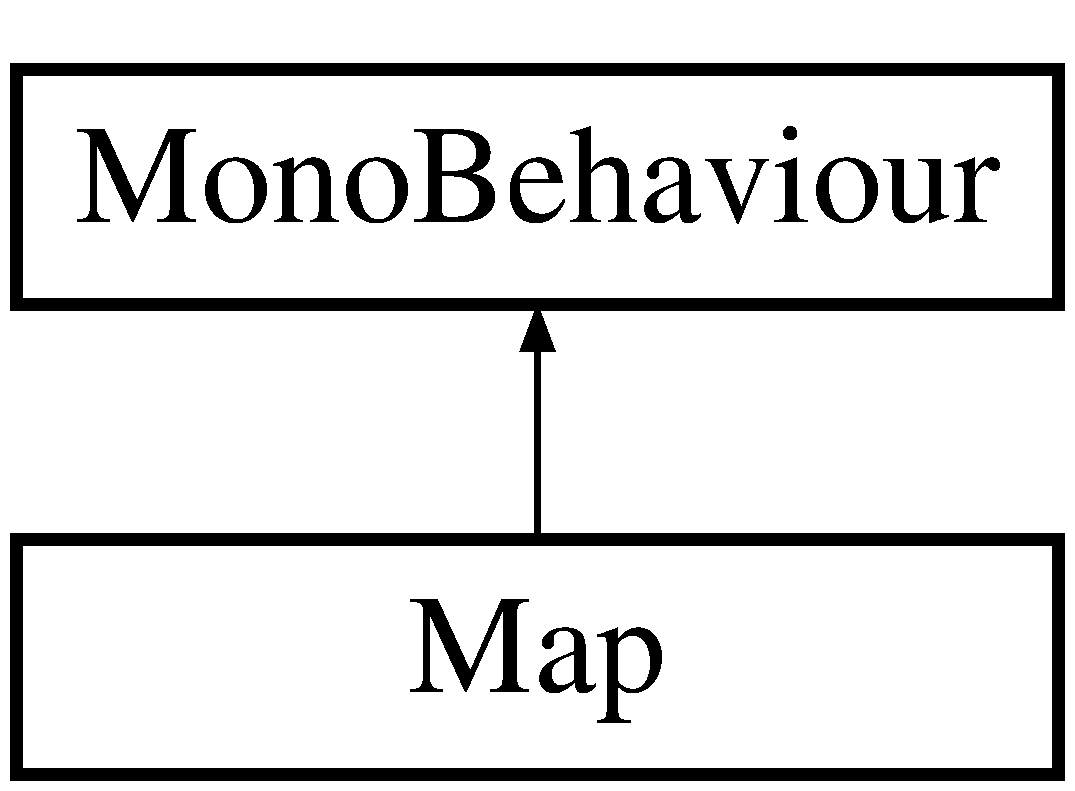
\includegraphics[height=2.000000cm]{class_map}
\end{center}
\end{figure}
\subsection*{Public Member Functions}
\begin{DoxyCompactItemize}
\item 
Transform \mbox{\hyperlink{class_map_a65f298678747e49b6f99ba46271e2519}{Get\+Board\+Holder}} ()
\item 
void \mbox{\hyperlink{class_map_a4b4925269b22d09fc07109d19f8c32e6}{place\+Floors}} ()
\item 
void \mbox{\hyperlink{class_map_a861230d1abdb5ed46e9dc95e8bf61d41}{place\+Walls}} ()
\item 
void \mbox{\hyperlink{class_map_a61d3bb5dbaec40d06efb1b29539f3d2f}{Map\+Setup}} (int cols, int row)
\end{DoxyCompactItemize}
\subsection*{Public Attributes}
\begin{DoxyCompactItemize}
\item 
\mbox{\Hypertarget{class_map_a284e57bb463795f868d0004f2c91ce34}\label{class_map_a284e57bb463795f868d0004f2c91ce34}} 
Game\+Object \mbox{[}$\,$\mbox{]} {\bfseries floor\+Tiles}
\item 
\mbox{\Hypertarget{class_map_abc75d741038130d7b274d5eab51758c1}\label{class_map_abc75d741038130d7b274d5eab51758c1}} 
Game\+Object \mbox{[}$\,$\mbox{]} {\bfseries wall\+Tiles}
\item 
\mbox{\Hypertarget{class_map_a9be8c4808419f525ab5452f1b074c90f}\label{class_map_a9be8c4808419f525ab5452f1b074c90f}} 
List$<$ Vector3 $>$ {\bfseries grid\+Positions} = new List $<$Vector3$>$ ()
\item 
\mbox{\Hypertarget{class_map_a4a5808c38dec273b158a81a6af47e5f5}\label{class_map_a4a5808c38dec273b158a81a6af47e5f5}} 
List$<$ Vector3 $>$ {\bfseries floor\+Positions} = new List $<$Vector3$>$ ()
\item 
\mbox{\Hypertarget{class_map_a86f5dc6f831600a856ee693454bdf308}\label{class_map_a86f5dc6f831600a856ee693454bdf308}} 
int {\bfseries columns}
\item 
\mbox{\Hypertarget{class_map_a4c6ba6b1a6ba20821550e6dd8f8cefbe}\label{class_map_a4c6ba6b1a6ba20821550e6dd8f8cefbe}} 
int {\bfseries rows}
\end{DoxyCompactItemize}


\subsection{Member Function Documentation}
\mbox{\Hypertarget{class_map_a65f298678747e49b6f99ba46271e2519}\label{class_map_a65f298678747e49b6f99ba46271e2519}} 
\index{Map@{Map}!Get\+Board\+Holder@{Get\+Board\+Holder}}
\index{Get\+Board\+Holder@{Get\+Board\+Holder}!Map@{Map}}
\subsubsection{\texorpdfstring{Get\+Board\+Holder()}{GetBoardHolder()}}
{\footnotesize\ttfamily Transform Map.\+Get\+Board\+Holder (\begin{DoxyParamCaption}{ }\end{DoxyParamCaption})\hspace{0.3cm}{\ttfamily [inline]}}

Returns a holder in the hiearchy to hold walls, floor etc...  None  Transform \mbox{\Hypertarget{class_map_a61d3bb5dbaec40d06efb1b29539f3d2f}\label{class_map_a61d3bb5dbaec40d06efb1b29539f3d2f}} 
\index{Map@{Map}!Map\+Setup@{Map\+Setup}}
\index{Map\+Setup@{Map\+Setup}!Map@{Map}}
\subsubsection{\texorpdfstring{Map\+Setup()}{MapSetup()}}
{\footnotesize\ttfamily void Map.\+Map\+Setup (\begin{DoxyParamCaption}\item[{int}]{cols,  }\item[{int}]{row }\end{DoxyParamCaption})\hspace{0.3cm}{\ttfamily [inline]}}

sets the size of the map and calls Board\+Setup()  int cols  int row  None \mbox{\Hypertarget{class_map_a4b4925269b22d09fc07109d19f8c32e6}\label{class_map_a4b4925269b22d09fc07109d19f8c32e6}} 
\index{Map@{Map}!place\+Floors@{place\+Floors}}
\index{place\+Floors@{place\+Floors}!Map@{Map}}
\subsubsection{\texorpdfstring{place\+Floors()}{placeFloors()}}
{\footnotesize\ttfamily void Map.\+place\+Floors (\begin{DoxyParamCaption}{ }\end{DoxyParamCaption})\hspace{0.3cm}{\ttfamily [inline]}}

Place the foor tiles  None  None \mbox{\Hypertarget{class_map_a861230d1abdb5ed46e9dc95e8bf61d41}\label{class_map_a861230d1abdb5ed46e9dc95e8bf61d41}} 
\index{Map@{Map}!place\+Walls@{place\+Walls}}
\index{place\+Walls@{place\+Walls}!Map@{Map}}
\subsubsection{\texorpdfstring{place\+Walls()}{placeWalls()}}
{\footnotesize\ttfamily void Map.\+place\+Walls (\begin{DoxyParamCaption}{ }\end{DoxyParamCaption})\hspace{0.3cm}{\ttfamily [inline]}}

Place the wall tiles  None  None 

The documentation for this class was generated from the following file\+:\begin{DoxyCompactItemize}
\item 
Map.\+cs\end{DoxyCompactItemize}

%--- End generated contents ---

% Index
\backmatter
\newpage
\phantomsection
\clearemptydoublepage
\addcontentsline{toc}{chapter}{Index}
\printindex

\end{document}
